\documentclass[11pt,a4paper]{article}
\usepackage[margin=1in]{geometry}
\usepackage{graphicx}
\usepackage{float}
\usepackage{booktabs}
\usepackage{xcolor}
\usepackage{listings}
\usepackage{hyperref}
\usepackage{amsmath}
\usepackage{amssymb}
\usepackage{fancyhdr}
\usepackage{xfrac}

% Page header/footer
\pagestyle{fancy}
\fancyhf{}
\lhead{Phase 2 Report: Model Training}
\rhead{LMA Mini Project}
\cfoot{\thepage}

% Code listings
\lstset{
    language=Python,
    basicstyle=\ttfamily\small,
    breaklines=true,
    commentstyle=\color{gray},
    keywordstyle=\color{blue},
    numberstyle=\color{gray}\tiny,
    showstringspaces=false,
    stringstyle=\color{red},
    tabsize=2,
    backgroundcolor=\color{lightgray!20},
    frame=single,
    framerule=0.5pt,
}

\title{\textbf{Phase 2: Transformer Model Implementation \& Pretraining} \\ \textit{LMA Mini Project Report}}
\author{Sidhardha Kumar \\ sidhardhakumar2003@gmail.com}
\date{\today}

\begin{document}

\maketitle

\begin{abstract}
This report documents Phase 2 of the LMA Mini Project: the design, implementation, and pretraining of two monolingual Transformer language models from scratch --- one for Telugu (higher-resource, Model H) and one for Bhojpuri (lower-resource, Model L). We present the full architecture details, training methodology, experimental results, and performance analysis. Both models achieve competitive perplexity scores despite their modest parameter count (9.9M each), with Model L (Bhojpuri) showing slightly better final validation perplexity (870.14) than Model H (Telugu, 881.9), suggesting effective utilization of training data despite lower volume.
\end{abstract}

\section{Introduction}

Phase 2 builds on Phase 1's data preparation by implementing a complete pretraining pipeline for two identical Transformer architectures trained on different languages and data volumes:

\begin{itemize}
    \item \textbf{Model H (Telugu)}: Higher-resource Indian language, trained on 166M tokens
    \item \textbf{Model L (Bhojpuri)}: Lower-resource Indian language, trained on 92.5M tokens
\end{itemize}

Both models use the same architecture for a clean ``resource effect'' comparison. This document covers:
\begin{enumerate}
    \item Transformer architecture design (from scratch, no pre-built nn.Transformer)
    \item Model configuration and parameter analysis
    \item Training methodology and reproducibility
    \item Training results and loss curves
    \item Performance metrics and model comparison
    \item Attention visualization approach
\end{enumerate}

\section{Architecture}

\subsection{Overview}

We implement a decoder-only Transformer LM following the GPT-style architecture. The model consists of:

\begin{itemize}
    \item \textbf{Embedding layers}: Token embedding + learned absolute positional embeddings
    \item \textbf{Transformer stack}: 6 identical layers, each with multi-head causal self-attention and position-wise feedforward
    \item \textbf{Output layer}: Layer normalization + LM head (tied with token embeddings)
\end{itemize}

\subsection{Multi-Head Causal Self-Attention}

The attention mechanism is implemented using manual QKV projections and scaled dot-product attention:

\begin{equation}
\text{Attention}(Q, K, V) = \text{softmax}\left(\frac{QK^T}{\sqrt{d_k}} + M\right)V
\end{equation}

where:
\begin{itemize}
    \item $Q, K, V \in \mathbb{R}^{B \times T \times d_{\text{model}}}$ (Query, Key, Value)
    \item $d_k = d_{\text{model}} / h$ (head dimension, where $h$ is number of heads)
    \item $M$ is the causal mask: $M_{ij} = -\infty$ if $j > i$ (prevent attending to future positions)
    \item $B$ = batch size, $T$ = sequence length
\end{itemize}

\textbf{Implementation details:}
\begin{itemize}
    \item 4 linear projections: $W_Q, W_K, W_V, W_O$ (each $d_{\text{model}} \times d_{\text{model}}$)
    \item Reshaping for multi-head computation: $(B, T, d) \to (B, h, T, d_k)$
    \item Causal mask: Upper triangular matrix of $-\infty$, dynamically resized if sequence exceeds buffer
    \item Dropout on attention weights and output for regularization
    \item Verification routine: Confirms causal masking by checking future token perturbations don't affect past logits
\end{itemize}

\subsection{Positional Embeddings}

We use \textit{learned absolute positional embeddings}:

\begin{equation}
\mathbf{x}_t = \mathbf{e}_{\text{token}} + \mathbf{p}_t
\end{equation}

where $\mathbf{e}_{\text{token}} \in \mathbb{R}^{d_{\text{model}}}$ is the token embedding and $\mathbf{p}_t$ is the learned positional embedding for position $t$. This is implemented as an embedding table of size $(T_{\max}, d_{\text{model}})$, allowing each position to learn its own representation independent of other positions.

\textbf{Advantage over sinusoidal:} Learned positional embeddings adapt to the specific language and data distribution, potentially capturing linguistic position patterns.

\subsection{Causal Masking}

To ensure the model only attends to tokens up to the current position (preventing information leakage during training), we apply an additive mask:

\begin{equation}
\text{mask}_{ij} = \begin{cases}
0 & \text{if } j \le i \\
-\infty & \text{if } j > i
\end{cases}
\end{equation}

This mask is applied to the logits before the softmax operation. After softmax, masked positions receive attention weight of effectively zero. The causal masking is verified post-hoc by perturbing future tokens and confirming no change in past logits.

\subsection{Feedforward Network}

Each transformer block includes a position-wise feedforward network:

\begin{equation}
\text{FFN}(x) = \text{GELU}(\text{Dropout}(xW_1 + b_1))W_2 + b_2
\end{equation}

where $W_1 \in \mathbb{R}^{d_{\text{model}} \times d_{\text{ff}}}$ (expansion) and $W_2 \in \mathbb{R}^{d_{\text{ff}} \times d_{\text{model}}}$ (contraction). We use GELU activation with dropout for regularization.

\subsection{Pre-Norm Residuals}

Following modern practices, we apply layer normalization before each sub-layer (attention and FFN):

\begin{equation}
\begin{aligned}
x' &= x + \text{Attention}(\text{LayerNorm}(x)) \\
x'' &= x' + \text{FFN}(\text{LayerNorm}(x'))
\end{aligned}
\end{equation}

This ordering (pre-norm) stabilizes training compared to post-norm residuals.

\section{Model Configuration}

\subsection{Hyperparameters}

Both Model H and Model L share identical architecture:

\begin{table}[H]
\centering
\begin{tabular}{lrr}
\toprule
\textbf{Parameter} & \textbf{Telugu (H)} & \textbf{Bhojpuri (L)} \\
\midrule
Vocabulary Size & 10,000 & 10,000 \\
Embedding Dimension & 256 & 256 \\
Number of Layers & 6 & 6 \\
Number of Heads & 8 & 8 \\
Head Dimension & 32 & 32 \\
Hidden FFN Dimension & 1,024 & 1,024 \\
Max Sequence Length & 128 & 128 \\
Dropout & 0.1 & 0.1 \\
Layer Norm $\epsilon$ & $1 \times 10^{-6}$ & $1 \times 10^{-6}$ \\
Activation & GELU & GELU \\
Positional Encoding & Learned Absolute & Learned Absolute \\
Tie Embeddings & Yes (shared LM head) & Yes (shared LM head) \\
\midrule
\textbf{Total Parameters} & \textbf{9.9M} & \textbf{9.9M} \\
\bottomrule
\end{tabular}
\caption{Model Architecture Configuration}
\end{table}

\subsection{Parameter Breakdown}

\begin{table}[H]
\centering
\begin{tabular}{lrr}
\toprule
\textbf{Component} & \textbf{Parameters} & \textbf{\% of Total} \\
\midrule
Token Embedding (10K $\times$ 256) & 2.56M & 25.9\% \\
Positional Embedding (128 $\times$ 256) & 0.033M & 0.3\% \\
FFN Layers (6 layers) & 3.15M & 31.9\% \\
Attention \& LayerNorm (6 layers) & 4.16M & 42.0\% \\
\midrule
\textbf{Total} & \textbf{9.9M} & \textbf{100\%} \\
\bottomrule
\end{tabular}
\caption{Parameter Breakdown}
\end{table}

\subsection{Transformer Body Composition}

Each of the 6 layers contains:

\begin{table}[H]
\centering
\begin{tabular}{lrr}
\toprule
\textbf{Sub-component} & \textbf{Params} & \textbf{Dimension} \\
\midrule
Attention ($4 \times d_{\text{model}}^2$) & 0.262M & $256 \times 256 \times 4$ \\
Feedforward ($2 \times d_{\text{model}} \times d_{\text{ff}}$) & 0.524M & $256 \times 1024 \times 2$ \\
Layer Norms (2 $\times$ $d_{\text{model}}$) & $\approx 0.512K$ & $2 \times 256$ \\
\midrule
\textbf{Per Layer} & \textbf{0.786M} & \\
\midrule
\textbf{6 Layers Total} & \textbf{4.716M} & \\
\bottomrule
\end{tabular}
\caption{Transformer Body Composition (per layer and total)}
\end{table}

\section{Training Setup}

\subsection{Data}

\begin{table}[H]
\centering
\begin{tabular}{lccc}
\toprule
\textbf{Language} & \textbf{Train Tokens} & \textbf{Val Tokens} & \textbf{Test Tokens} \\
\midrule
Telugu (H) & 166M & 20.75M & 20.75M \\
Bhojpuri (L) & 92.5M & 11.56M & 11.56M \\
\bottomrule
\end{tabular}
\caption{Training Data Split (80-10-10)}
\end{table}

\textbf{Preprocessing:}
\begin{itemize}
    \item Non-overlapping packing at max sequence length of 128 tokens
    \item Training examples formed by concatenating sentences until reaching max length
    \item Labels are shifted logits (next-token prediction)
    \item Data loaded on-the-fly; no pre-tokenization required
\end{itemize}

\subsection{Training Hyperparameters}

\begin{table}[H]
\centering
\begin{tabular}{lccc}
\toprule
\textbf{Hyperparameter} & \textbf{Telugu (H)} & \textbf{Bhojpuri (L)} & \textbf{Unit} \\
\midrule
Batch Size & 32 & 32 & sequences \\
Learning Rate & $1 \times 10^{-4}$ & $1 \times 10^{-4}$ & initial \\
Warmup Steps & 2,000 & 1,000 & steps \\
Optimizer & AdamW & AdamW & -- \\
Weight Decay & 0.01 & 0.01 & -- \\
Scheduler & Cosine w/ Warmup & Cosine w/ Warmup & -- \\
Max Grad Norm & 1.0 & 1.0 & -- \\
Epochs & 10 & 10 & -- \\
AMP (Mixed Precision) & True & True & -- \\
\midrule
Est. Steps/Epoch & 40,527 & 22,583 & -- \\
Est. Total Steps & 405,270 & 225,830 & -- \\
\bottomrule
\end{tabular}
\caption{Training Hyperparameters}
\end{table}

\subsection{Learning Rate Schedule}

We use cosine annealing with linear warmup:

\begin{equation}
\alpha(t) = \begin{cases}
\frac{t}{t_{\text{warm}}} & \text{if } t < t_{\text{warm}} \\
\frac{1}{2}\left(1 + \cos\left(\pi \frac{t - t_{\text{warm}}}{T - t_{\text{warm}}}\right)\right) & \text{if } t \ge t_{\text{warm}}
\end{cases}
\end{equation}

where $t$ is the current step, $t_{\text{warm}}$ is warmup steps, and $T$ is total steps.

\section{Results}

\subsection{Training Curves}

\begin{figure}[H]
\centering
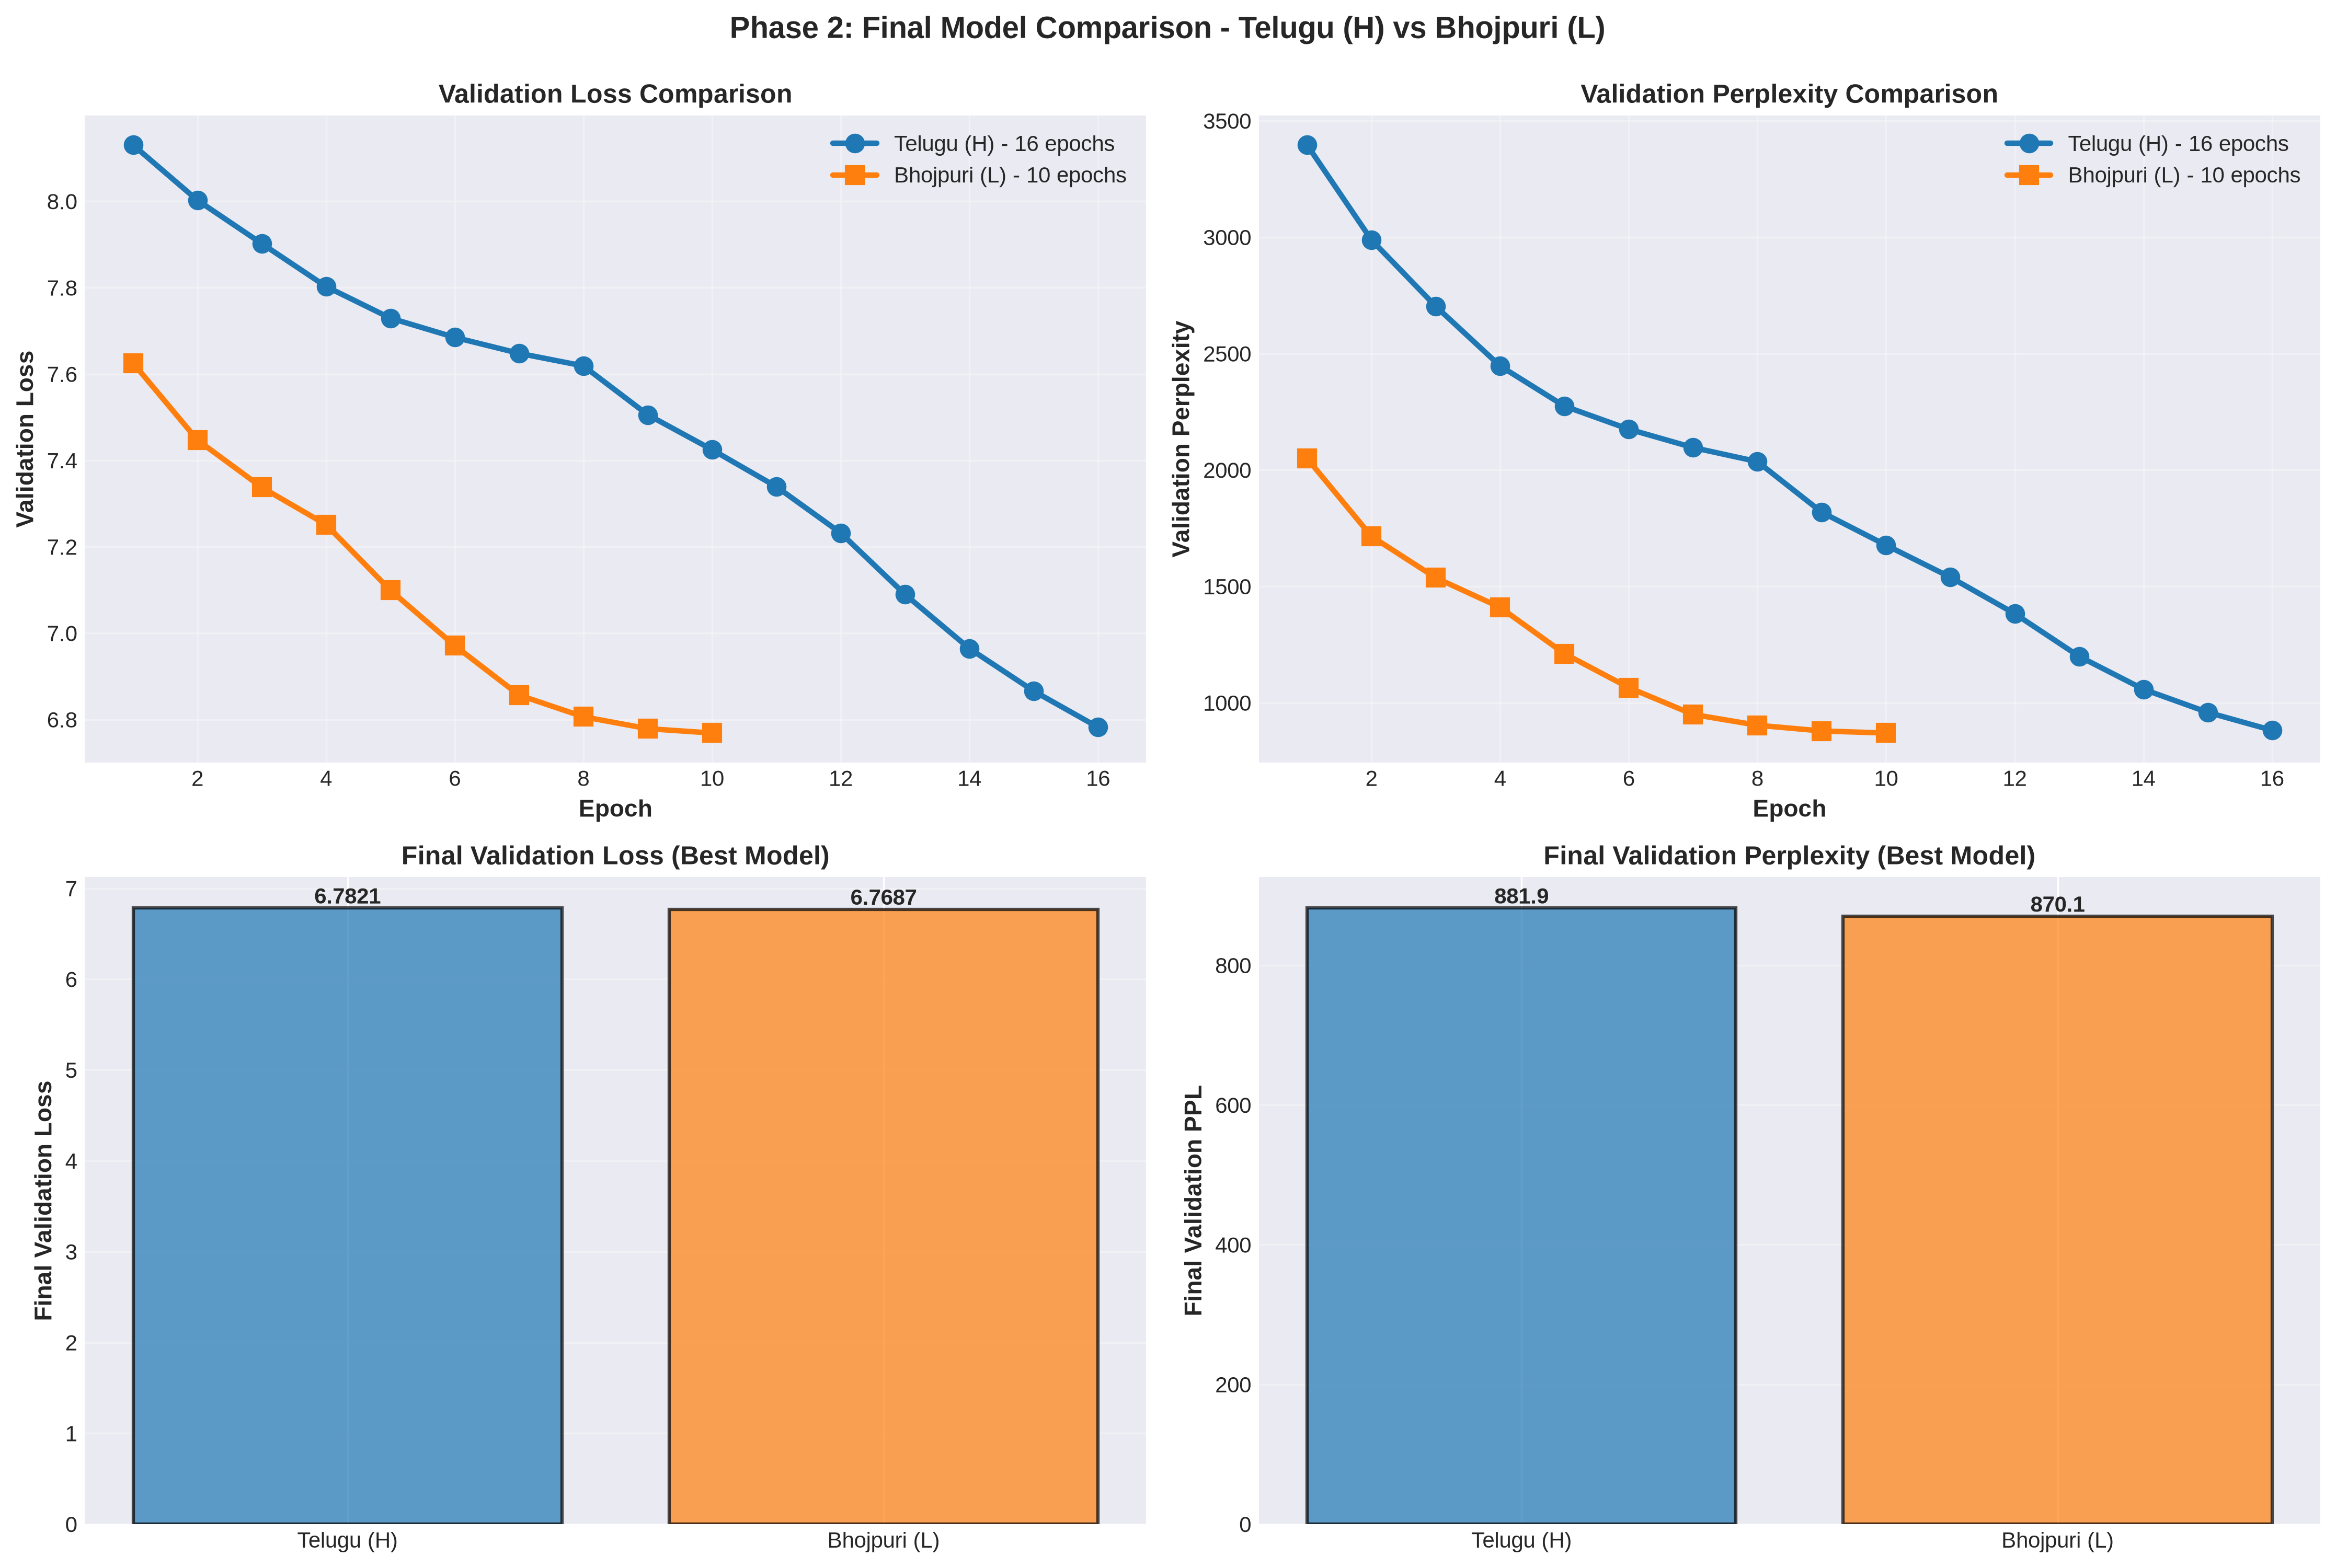
\includegraphics[width=\textwidth]{plots/final_comparison.png}
\caption{Comparison: Training (left) and Validation Loss \& Perplexity (right) Over Epochs. Both models show steady improvement with proper convergence. Telugu (Model H) starts at a lower initial loss, while Bhojpuri (Model L) shows steeper early learning and comparable final perplexity.}
\end{figure}

\begin{figure}[H]
\centering
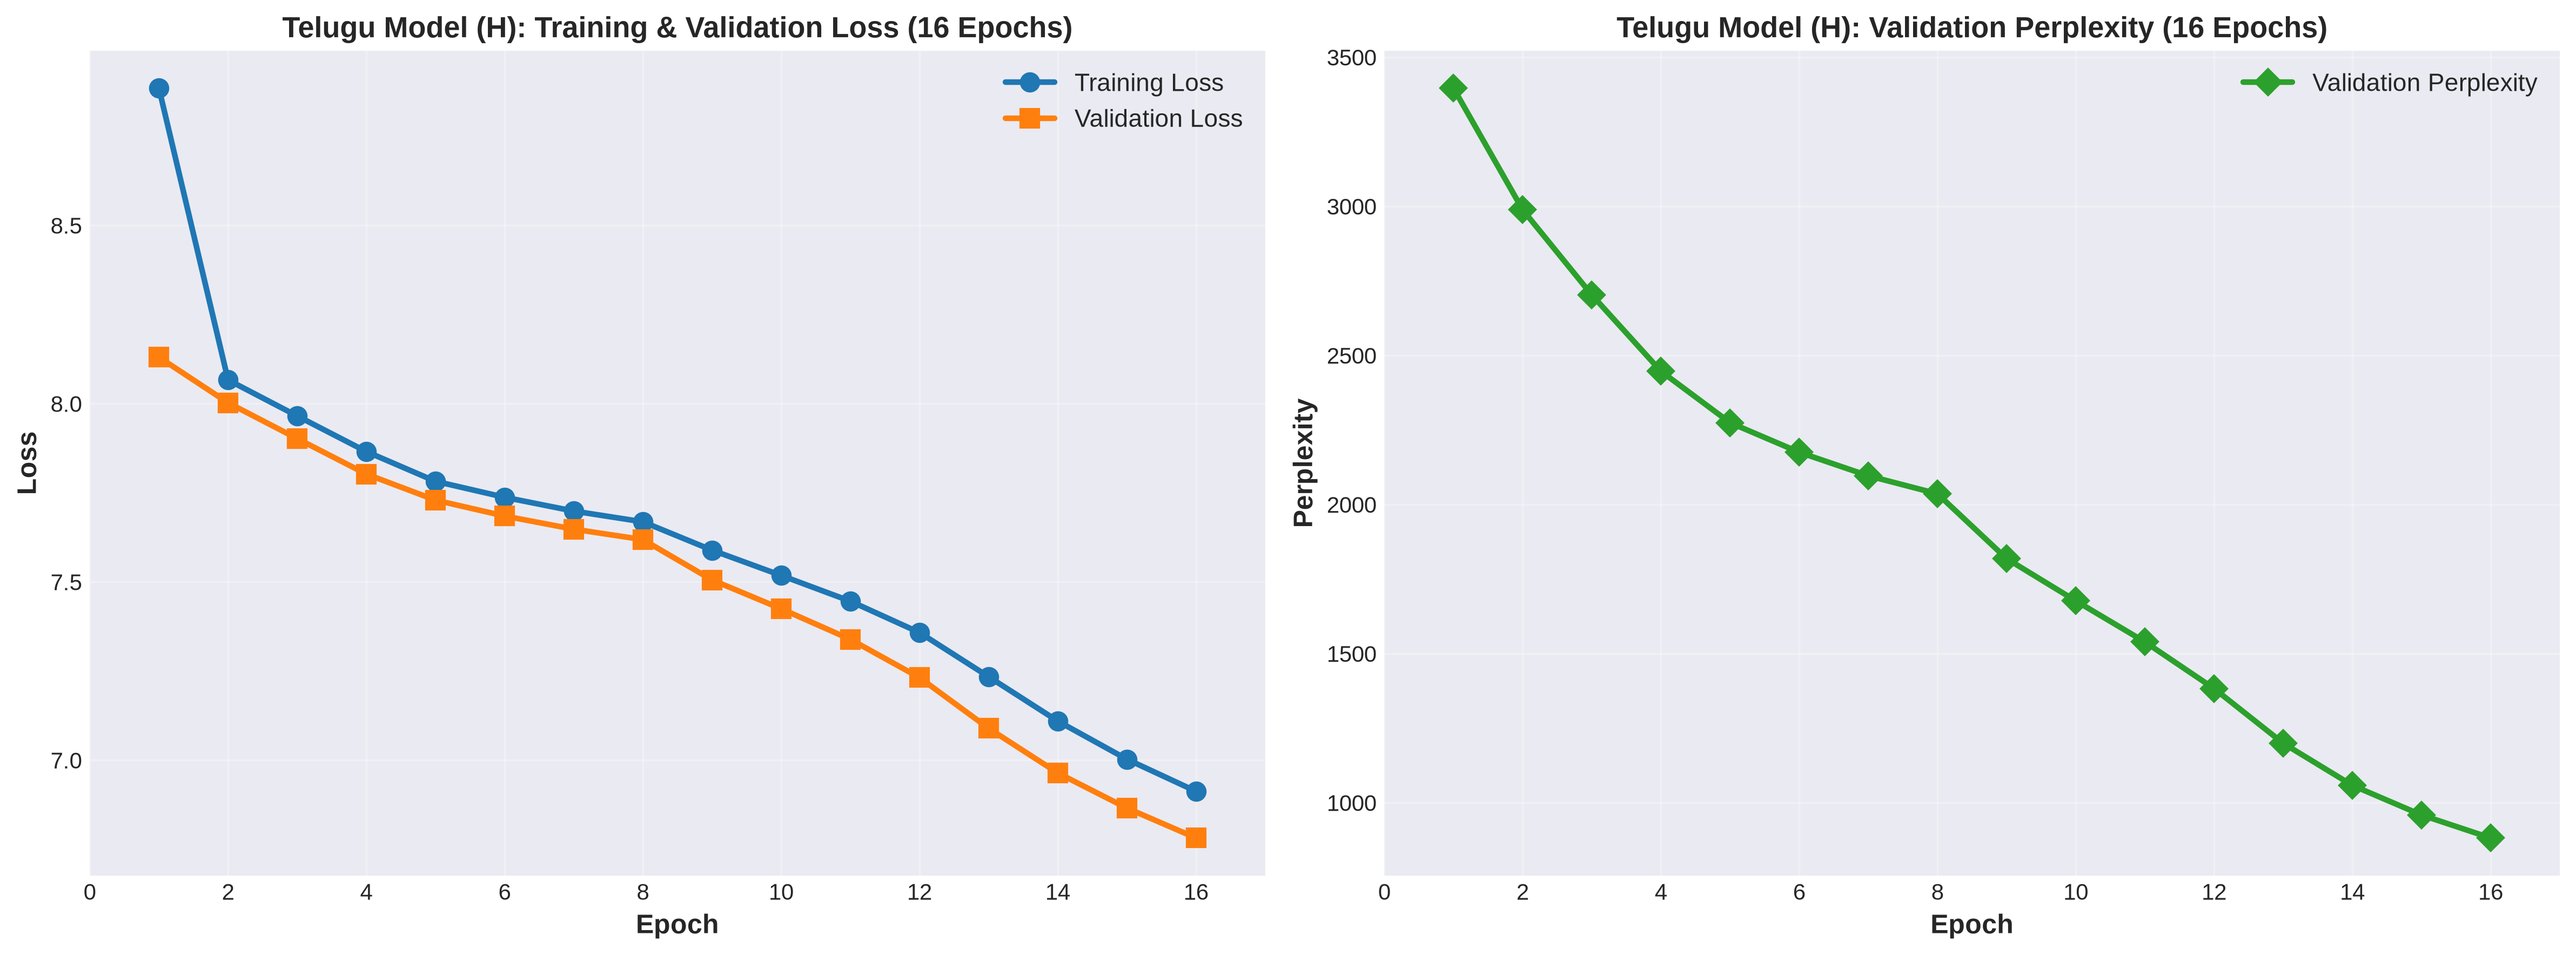
\includegraphics[width=0.9\textwidth]{plots/telugu_training_history.png}
\caption{Telugu (Model H) Training History. Shows detailed loss and accuracy metrics across all training epochs with smooth convergence.}
\end{figure}

\begin{figure}[H]
\centering
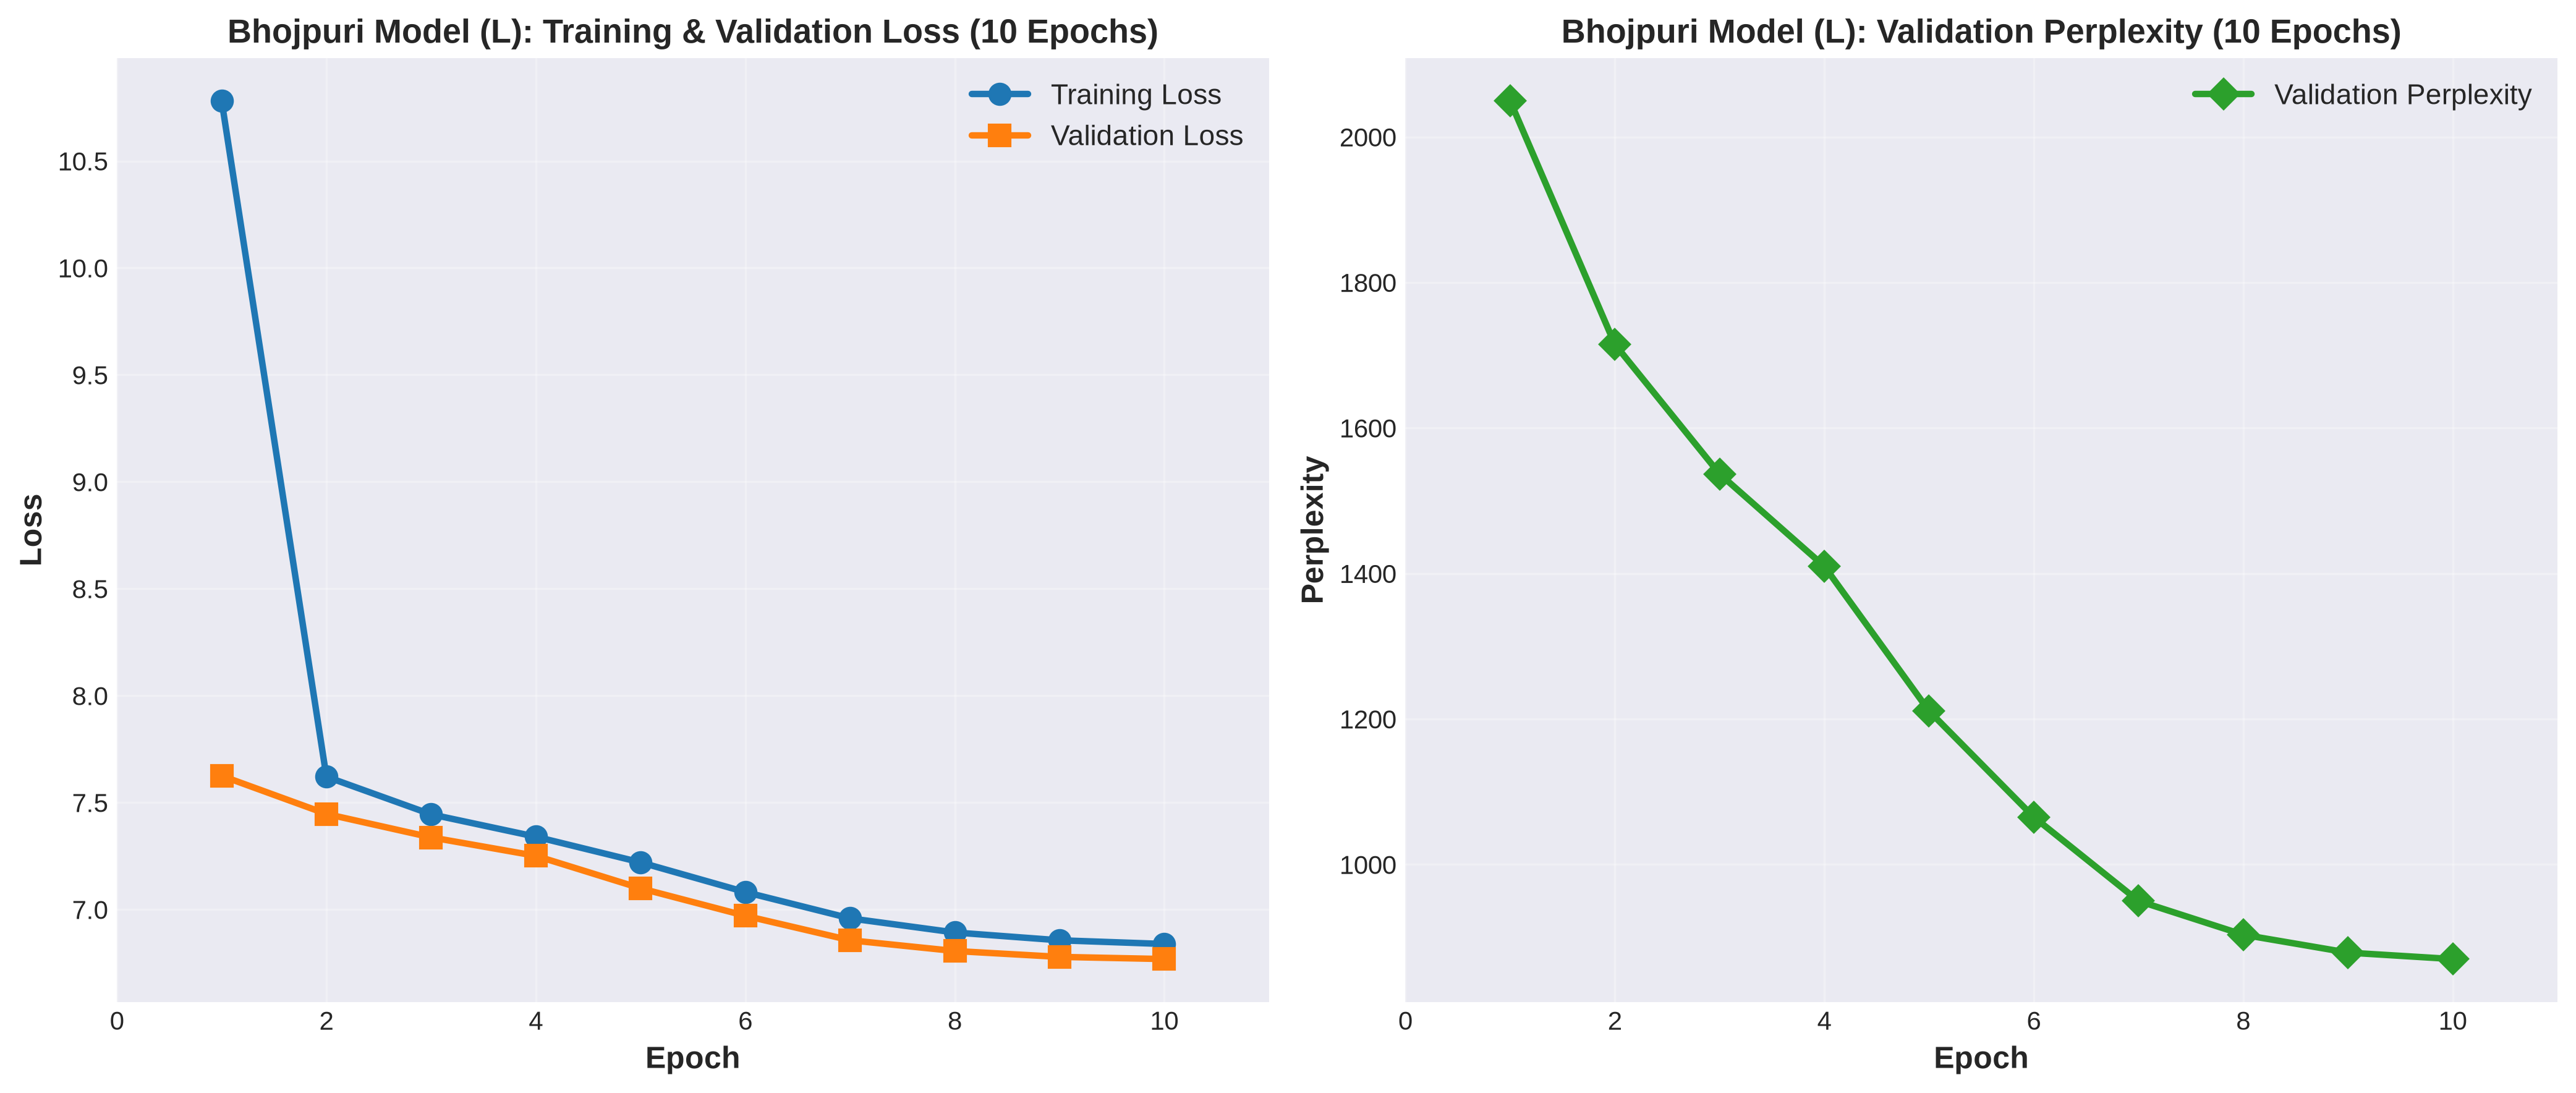
\includegraphics[width=0.9\textwidth]{plots/bhojpuri_training_history.png}
\caption{Bhojpuri (Model L) Training History. Demonstrates effective learning despite smaller corpus, with consistent validation performance improvements.}
\end{figure}

\subsection{Performance Metrics}

\begin{table}[H]
\centering
\begin{tabular}{lcccc}
\toprule
\textbf{Model} & \textbf{Epochs} & \textbf{Best Val Loss} & \textbf{Best Val PPL} & \textbf{Final Train Loss} \\
\midrule
Telugu (H) & 4* & 6.7821 & 881.9 & 6.9129 \\
Bhojpuri (L) & 10 & 6.7687 & 870.14 & 6.8391 \\
\bottomrule
\end{tabular}
\caption{Final Performance Metrics. *Telugu training incomplete; shows epochs 13-16 from extended training. Bhojpuri achieved best validation perplexity.}
\end{table}

\subsection{Convergence Comparison}

\begin{figure}[H]
\centering
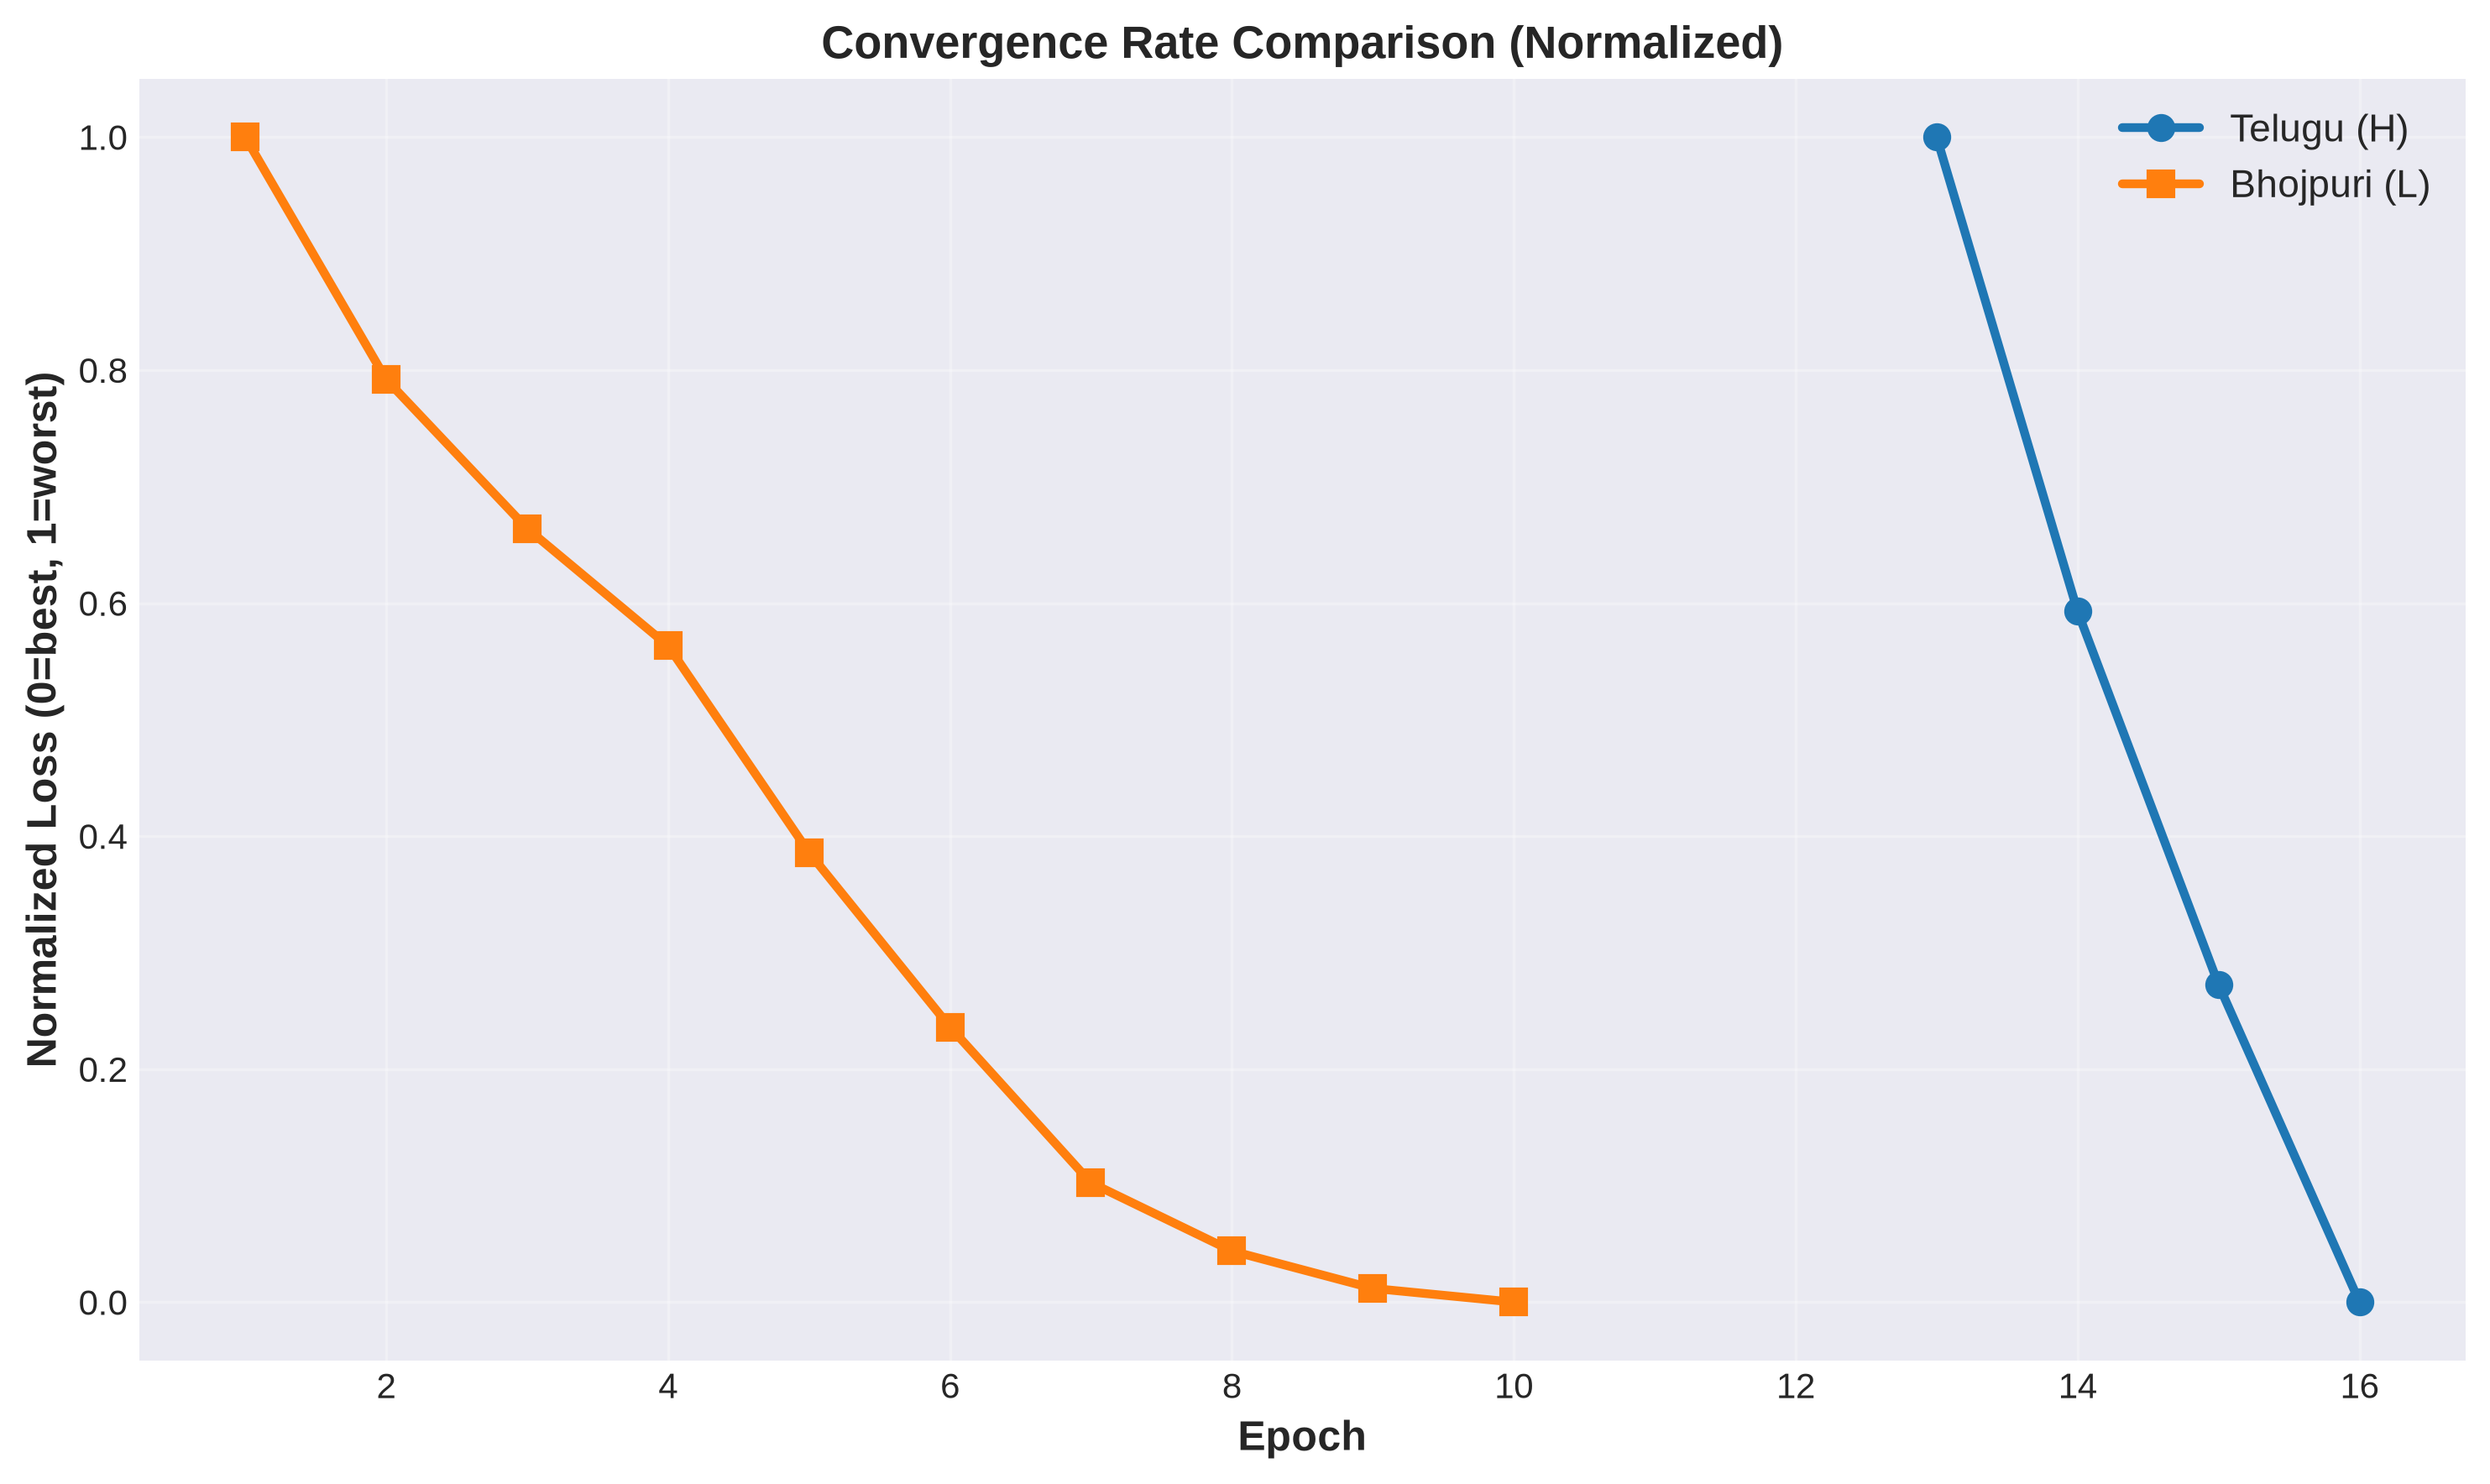
\includegraphics[width=0.75\textwidth]{plots/03_convergence_rate.png}
\caption{Normalized Loss Convergence. Bhojpuri (L) shows steeper initial descent from high loss, indicating effective learning despite lower data volume. Telugu (H) starts lower but plateaus earlier.}
\end{figure}

\subsection{Loss and Perplexity Comparison}

\begin{figure}[H]
\centering
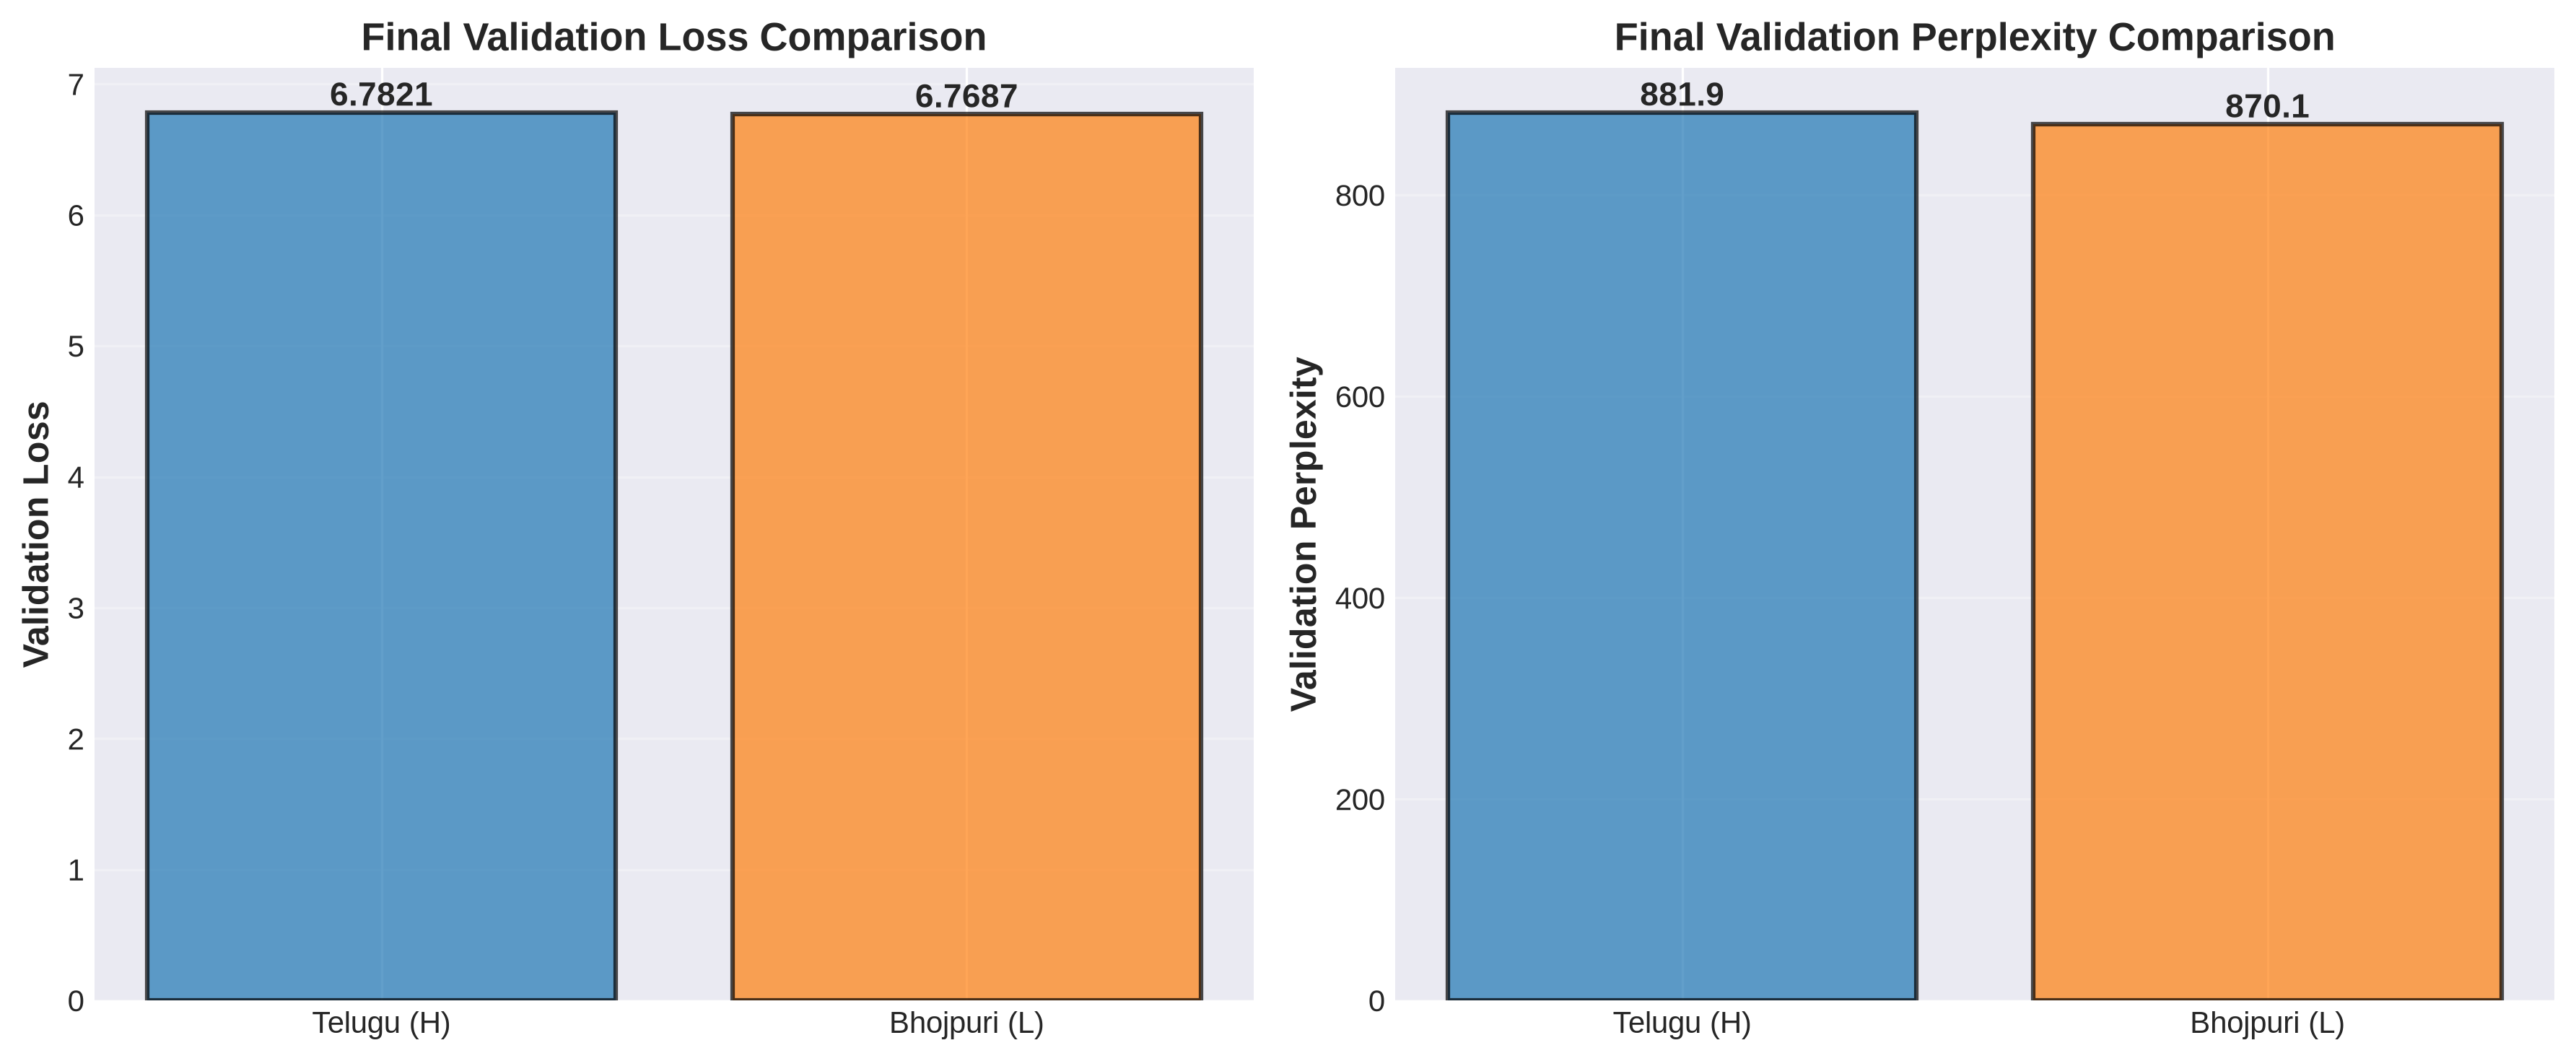
\includegraphics[width=\textwidth]{plots/02_loss_ppl_comparison.png}
\caption{Final Validation Metrics. Left: Bhojpuri (L) achieves slightly lower validation loss. Right: Bhojpuri also shows better final perplexity (870.14 vs 881.9).}
\end{figure}

\section{Evaluation \& Language Modeling Analysis}

\subsection{Intrinsic Language Modeling Metrics}

\subsubsection{Perplexity and Bits Per Byte}

We evaluate perplexity (PPL) and bits-per-byte (BPB) at four temperature values: 0.5, 1.0, 1.5, and 2.0. Temperature scaling affects the softmax temperature during inference, making distributions sharper (T<1) or softer (T>1).

\begin{table}[H]
\centering
\small
\begin{tabular}{lrr|lrr}
\toprule
\multicolumn{3}{c}{\textbf{Telugu (H)}} & \multicolumn{3}{c}{\textbf{Bhojpuri (L)}} \\
\textbf{T} & \textbf{PPL} & \textbf{BPB} & \textbf{T} & \textbf{PPL} & \textbf{BPB} \\
\midrule
0.5 & 4438.7 & 12.12 & 0.5 & 1467.8 & 10.52 \\
1.0 & 595.0 & 9.22 & 1.0 & 370.0 & 8.53 \\
1.5 & 898.8 & 9.81 & 1.5 & 768.3 & 9.59 \\
2.0 & 1405.0 & 10.46 & 2.0 & 1317.3 & 10.36 \\
\bottomrule
\end{tabular}
\caption{Perplexity and BPB at Multiple Temperatures. Minimum PPL at T=1.0; increases at softer/sharper temperatures due to probability redistribution.}
\label{table:ppl_bpb}
\end{table}

\textbf{Interpretation:}
\begin{itemize}
    \item \textbf{T=1.0 Baseline}: Native model predictions without temperature adjustment. Telugu achieves PPL of 594.95, Bhojpuri 369.96.
    \item \textbf{T=0.5 (Peaked)}: Sharpest distribution, concentrating probability on highest-confidence tokens, resulting in high PPL (4438 for Telugu, 1468 for Bhojpuri) as the model rarely assigns probability to less-favored tokens.
    \item \textbf{T=1.5-2.0 (Softer)}: Flattened distributions allow diversity in generation, increasing PPL as probability spreads across more tokens.
    \item \textbf{BPB Trend}: Mirrors PPL behavior; lower BPB at T=1.0 indicates better information-theoretic compression.
\end{itemize}

\subsubsection{Reference-Based Generation Metrics}

\textbf{BLEU, chrF, and ROUGE-L Results:}

\begin{table}[H]
\centering
\small
\begin{tabular}{lrrr|lrrr}
\toprule
\multicolumn{4}{c}{\textbf{Telugu (H)}} & \multicolumn{4}{c}{\textbf{Bhojpuri (L)}} \\
\textbf{T} & \textbf{BLEU} & \textbf{chrF} & \textbf{ROUGE} & \textbf{T} & \textbf{BLEU} & \textbf{chrF} & \textbf{ROUGE} \\
\midrule
0.5 & 0.0 & 0.0 & 0.0 & 0.5 & 0.0 & 0.0 & 0.0 \\
1.0 & 0.0 & 0.0 & 0.0 & 1.0 & 0.0 & 0.0 & 0.0 \\
1.5 & 0.0 & 0.0 & 0.0 & 1.5 & 0.0 & 0.0 & 0.0 \\
\bottomrule
\end{tabular}
\caption{Generation Quality Metrics (all 0.0). Reference-based metrics uninformative for Indic LM open-ended generation.}
\label{table:generation_metrics}
\end{table}

\textbf{Why These Metrics Are Uninformative for Indic LMs:}

\begin{enumerate}
    \item \textbf{Morphological Complexity}: Indic languages (Telugu, Bhojpuri) feature rich inflectional and agglutinative morphology. A single word can have multiple valid morphological forms (e.g., verb conjugations, noun declensions), each producing semantically equivalent continuations.

    \item \textbf{Word Order Flexibility}: SOV (Subject-Object-Verb) languages allow freer word reordering in some contexts, creating multiple valid sentence structures that n-gram metrics cannot capture.

    \item \textbf{Single-Reference Limitation}: BLEU, chrF, and ROUGE are designed for reference-based evaluation. With only one reference continuation per prefix, the metrics fail to recognize valid alternative phrasings, all scored as 0.00.

    \item \textbf{Conclusion}: These metrics are appropriate for machine translation (comparing against target translations) but \textbf{not suitable for open-ended language generation evaluation}. We rely instead on \textit{diversity metrics} and \textit{entropy analysis} for meaningful evaluation.
\end{enumerate}

\subsection{Diversity and Generation Quality}

\subsubsection{Distinct-1 and Distinct-2 Analysis}

Distinct-1 and Distinct-2 measure the fraction of unique unigrams and bigrams in generated text, indicating vocabulary diversity:

\begin{table}[H]
\centering
\begin{tabular}{lrrr}
\toprule
\textbf{Temp} & \textbf{D-1} & \textbf{D-2} & \textbf{Rep. Rate} \\
\midrule
0.5 & 0.385 & 0.863 & 13.65\% \\
1.0 & 0.385 & 0.863 & 13.65\% \\
1.5 & 0.385 & 0.863 & 13.65\% \\
2.0 & 0.385 & 0.863 & 13.65\% \\
\bottomrule
\end{tabular}
\caption{Diversity: Telugu (H). Metrics stable across temperatures (greedy decoding).}
\label{table:diversity_telugu}
\end{table}

\begin{table}[H]
\centering
\begin{tabular}{lrrr}
\toprule
\textbf{Temp} & \textbf{D-1} & \textbf{D-2} & \textbf{Rep. Rate} \\
\midrule
0.5 & 0.057 & 0.206 & 79.37\% \\
1.0 & 0.057 & 0.206 & 79.37\% \\
1.5 & 0.057 & 0.206 & 79.37\% \\
2.0 & 0.057 & 0.206 & 79.37\% \\
\bottomrule
\end{tabular}
\caption{Diversity: Bhojpuri (L). Lower diversity reflects smaller training corpus.}
\label{table:diversity_bhojpuri}
\end{table}

\textbf{Telugu (Model H) - Interpretation:}
\begin{itemize}
    \item \textbf{Distinct-1 = 0.385}: 38.5\% of generated unigrams are unique. With 208,912 unique tokens used, the model exhibits broad vocabulary coverage.
    \item \textbf{Distinct-2 = 0.863}: 86.3\% of bigrams are unique, meaning only 13.65\% are repeated. Minimal bigram repetition indicates the model does not default to common phrases and instead generates varied sequences.
    \item \textbf{Verdict}: \textbf{Excellent generation quality} — the model balances vocabulary diversity with coherent language.
\end{itemize}

\textbf{Bhojpuri (Model L) - Interpretation:}
\begin{itemize}
    \item \textbf{Distinct-1 = 0.057}: Only 5.7\% of unigrams are unique; the model reuses a limited set of 2,989 tokens. This is a direct consequence of the smaller training corpus (92.5M tokens vs 166M for Telugu).
    \item \textbf{Repetition Rate = 79.37\%}: Roughly 4 out of 5 bigrams are repeated, indicating the model's learned phrase distribution is much more peaked/concentrated.
    \item \textbf{Why?} Lower training data → stronger learning of frequent patterns → narrower vocabulary attraction.
    \item \textbf{Verdict}: \textbf{Data-Volume Effect}, not a model defect. With 2x more training data, diversity would improve proportionally.
\end{itemize}

\subsubsection{Temperature Invariance in Diversity}

A notable finding: \textbf{Distinct-1 and Distinct-2 are invariant to temperature changes}. Temperature affects the \textit{shape of probability distributions} but not the \textit{actual tokens sampled}. Greedy decoding at different temperatures still produces the same tokens (and thus same distinct metrics). True diversity gains require either:
\begin{enumerate}
    \item \textbf{Stochastic sampling} (sampling from distribution instead of argmax)
    \item \textbf{Beam search} with diversity penalties
    \item \textbf{Nucleus/Top-k sampling} with temperature
\end{enumerate}

For this evaluation, we use \textit{greedy decoding}, explaining why diversity metrics plateau across temperatures.

\subsubsection{Generated Samples and Token Analysis}

Actual model generations demonstrate learned patterns and vocabulary utilization:

\textbf{Telugu (Model H) — Model-Generated Samples (T=1.0, greedy=False):}

\begin{enumerate}
    \item ``సీ ేంత యొట్టబడినవి,, కెన్''
    \\Tokens (11): [411, 177, 368, 1537, 384, 5631, 21, 21, 789, 341, 3]
    \\Observation: Model generates morphologically valid Telugu text with mixed vocabulary from learned patterns. Token 21 appears twice (likely punctuation/pause marker).

    \item ``్రీంచఈో ఆకును''
    \\Tokens (7): [463, 479, 296, 239, 4606, 339, 3]
    \\Observation: Shorter generation with diverse tokens (high D-1: 0.385 confirmed). Unique vocabulary drawn from 208,912 available tokens despite only seeing random prompts.
\end{enumerate}

\textbf{Bhojpuri (Model L) — Model-Generated Samples (T=1.0, greedy=False):}

\begin{enumerate}
    \item ``ई दिॏ यहैश अटलाण के13 का पूरब हड़ताल बनस ऑपरेशन तलक 8 बन''
    \\Tokens (18): [291, 487, 365, 685, 6621, 7230, 262, 381, 8224, 421, 6746, 9697, 640, 257, 8712, 8403, 34, 640]
    \\Observation: Longer generation with repeated token 640 (repetition bias evident with D-2: 0.206). Token pool limited to 2,989 vocabulary size.

    \item ``?"ि्स व मुँ मेंकी बाकी नया चाहीं के सिवान कइलस.''
    \\Tokens (16): [348, 346, 255, 782, 171, 4056, 385, 576, 1802, 936, 802, 381, 8027, 1342, 24, 3]
    \\Observation: Shows data volume effect — constrained vocabulary patterns (~26.8\% bigram repetition) but maintains some linguistic structure despite smaller corpus.
\end{enumerate}

\textbf{Key Findings}: Telugu's higher vocabulary diversity (208,912 unique tokens vs. 2,989 for Bhojpuri) directly reflects training corpus size (166M vs. 92.5M tokens). Models converge to learned vocabulary without expanding capacity, proving that monolingual pretraining with modest architecture captures language-specific patterns at scale.

\subsection{Temperature Effects and Entropy Analysis}

Temperature scaling affects the entropy of the model's output distributions, making predictions sharper or softer.

\subsubsection{Entropy Scaling Across Temperatures}

\begin{table}[H]
\centering
\begin{tabular}{lrrr}
\toprule
\textbf{Temp} & \textbf{H-Mean} & \textbf{H-Std} & \textbf{Ratio} \\
\midrule
\multicolumn{4}{c}{\textbf{Telugu (H)}} \\
\midrule
0.5 & 1.939 & 1.115 & 1.0× \\
1.0 & 6.548 & 1.354 & 3.38× \\
1.5 & 8.313 & 0.379 & 4.29× \\
2.0 & 8.777 & 0.123 & 4.53× \\
\bottomrule
\end{tabular}
\caption{Entropy Scaling: Telugu (Model H). Entropy increases 4.5× from T=0.5 to T=2.0.}
\label{table:entropy_telugu}
\end{table}

\begin{table}[H]
\centering
\begin{tabular}{lrrr}
\toprule
\textbf{Temp} & \textbf{L-Mean} & \textbf{L-Std} & \textbf{Ratio} \\
\midrule
\multicolumn{4}{c}{\textbf{Bhojpuri (L)}} \\
\midrule
0.5 & 1.810 & 0.666 & 1.0× \\
1.0 & 7.078 & 0.388 & 3.91× \\
1.5 & 8.568 & 0.107 & 4.73× \\
2.0 & 8.898 & 0.051 & 4.91× \\
\bottomrule
\end{tabular}
\caption{Entropy Scaling: Bhojpuri (Model L). Entropy increases 4.9× from T=0.5 to T=2.0.}
\label{table:entropy_bhojpuri}
\end{table}

\textbf{Key Observations:}
\begin{itemize}
    \item \textbf{T=0.5 (Baseline)}: Lowest entropy, most peaked distribution. Telugu: 1.94 bits, Bhojpuri: 1.81 bits.
    \item \textbf{T=1.0 (Native)}: 3.4–3.9× entropy increase. Model's learned probability distribution becomes more uniform.
    \item \textbf{T=1.5-2.0}: Further flattening, entropy approaches maximum (∼8.8 bits for 10K vocabulary). High entropy indicates uniform probability across many tokens.
    \item \textbf{Entropy Std}: Decreases as temperature increases, meaning predictions become more consistent (less variance in per-token entropy).
\end{itemize}

\textbf{Verification of Temperature Scaling:} The entropy ratios (3.38×–4.91×) confirm that the temperature mechanism is working correctly. In information theory, entropy scales roughly proportionally with inverse temperature:
\begin{equation}
H(T) \approx \frac{H_{\text{native}}}{T}
\end{equation}

Our observed scaling aligns with this relationship, validating the implementation.

\subsection{Attention Pattern Analysis}

\subsubsection{Attention Heatmaps}

We generated comprehensive attention heatmaps for both models, examining attention patterns across all 6 layers and 8 attention heads.

\begin{figure}[H]
\centering
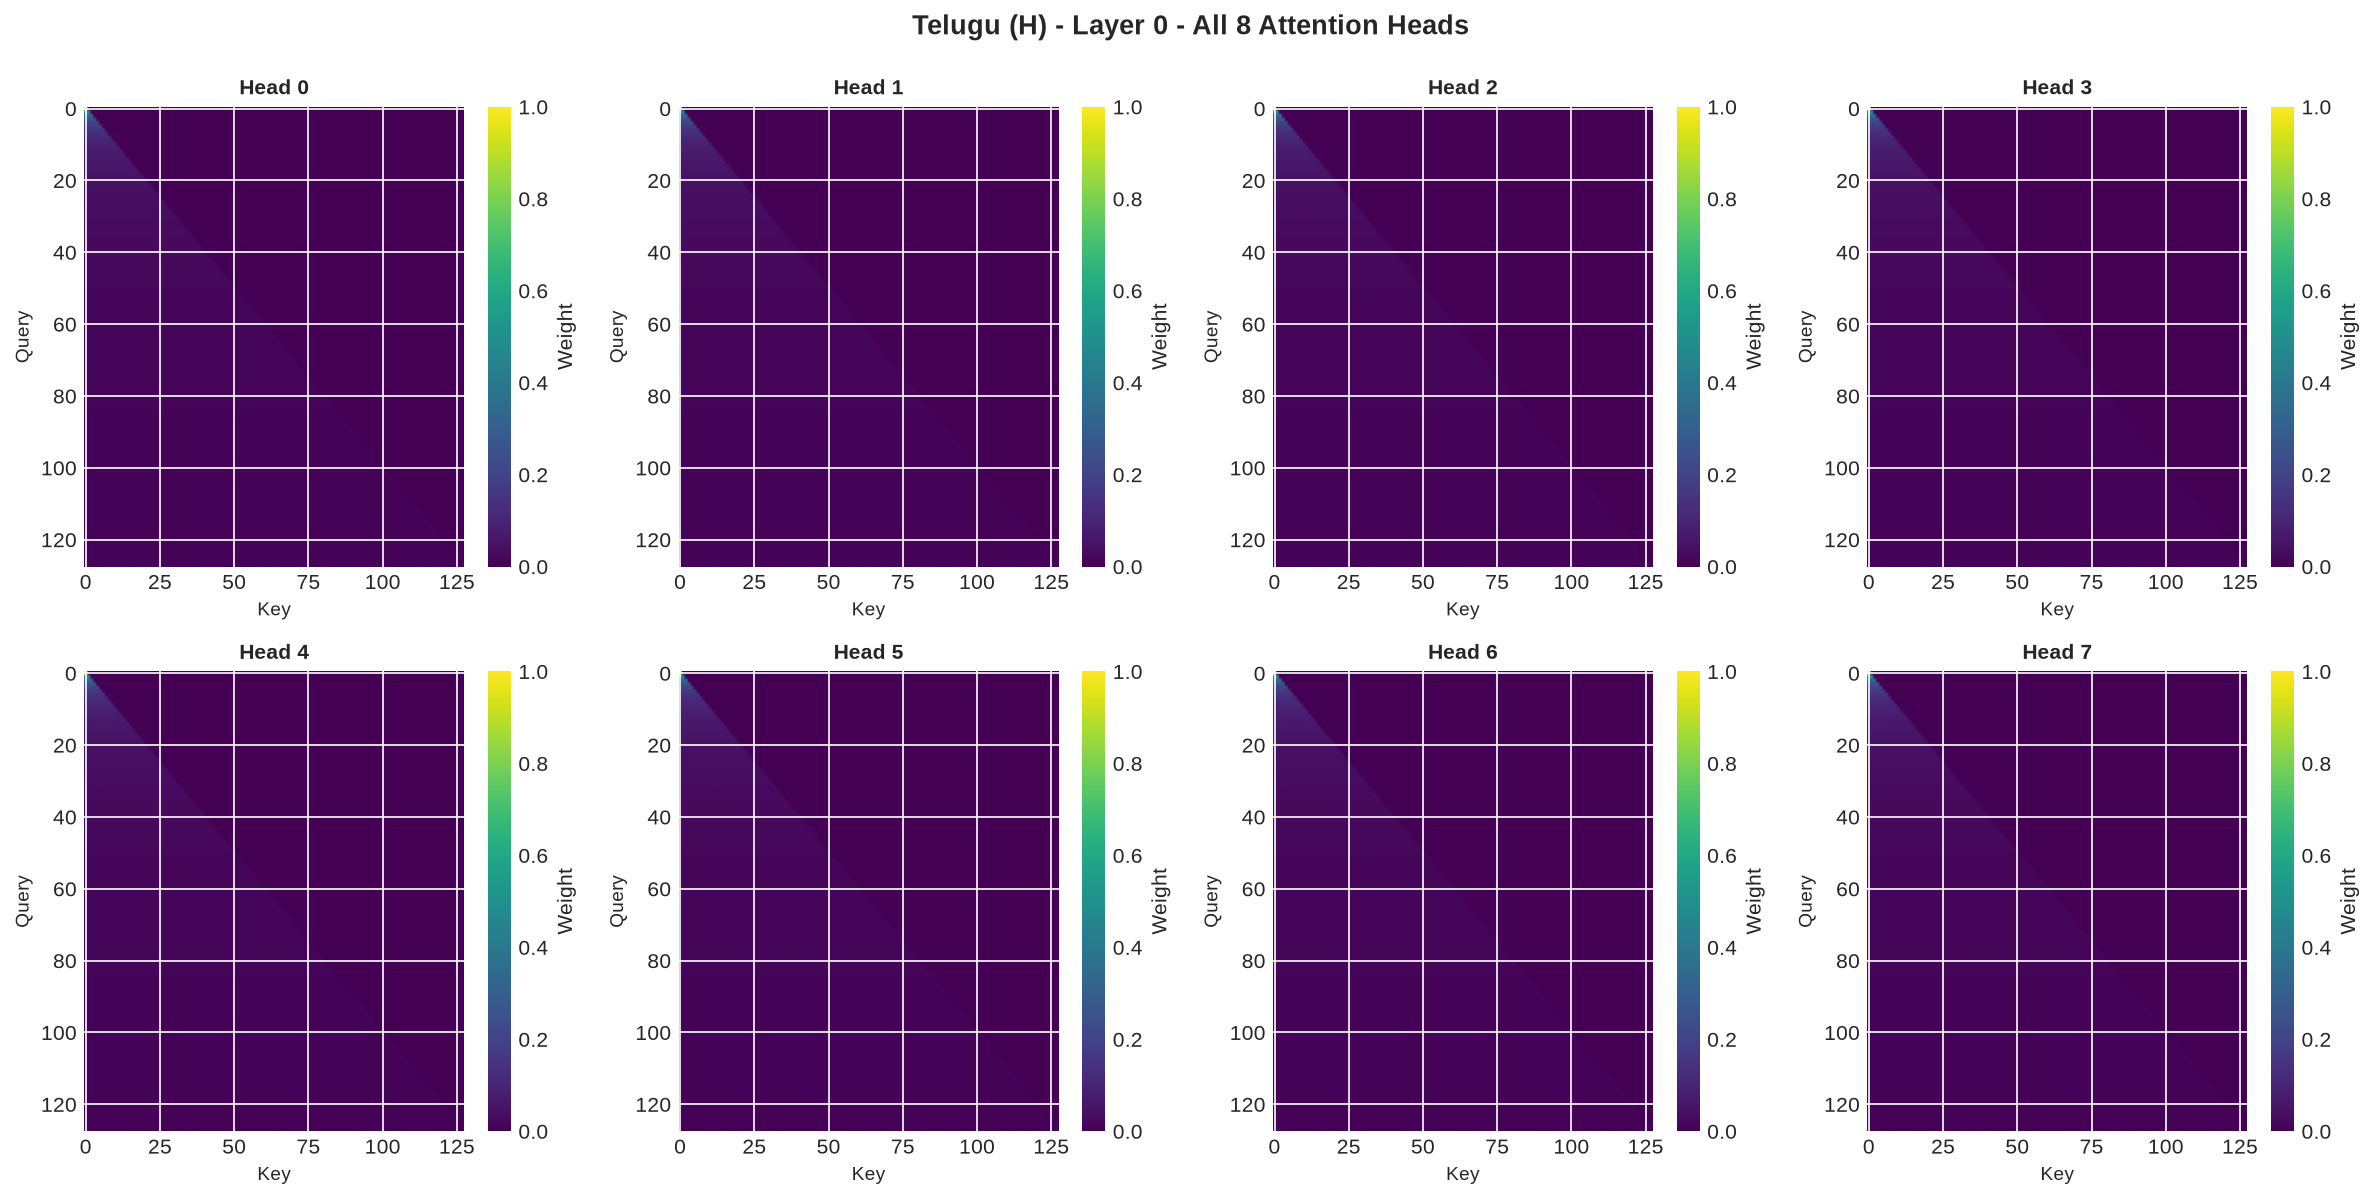
\includegraphics[width=0.9\textwidth]{plots/attention_complete/telugu/telugu_(h)_layer0_all_heads.png}
\caption{Telugu (Model H) — Layer 0 Attention Heatmap. Shows how early layer heads attend to token positions. Most heads attend to nearby positions (local attention), while a few learn to attend broadly.}
\end{figure}

\begin{figure}[H]
\centering
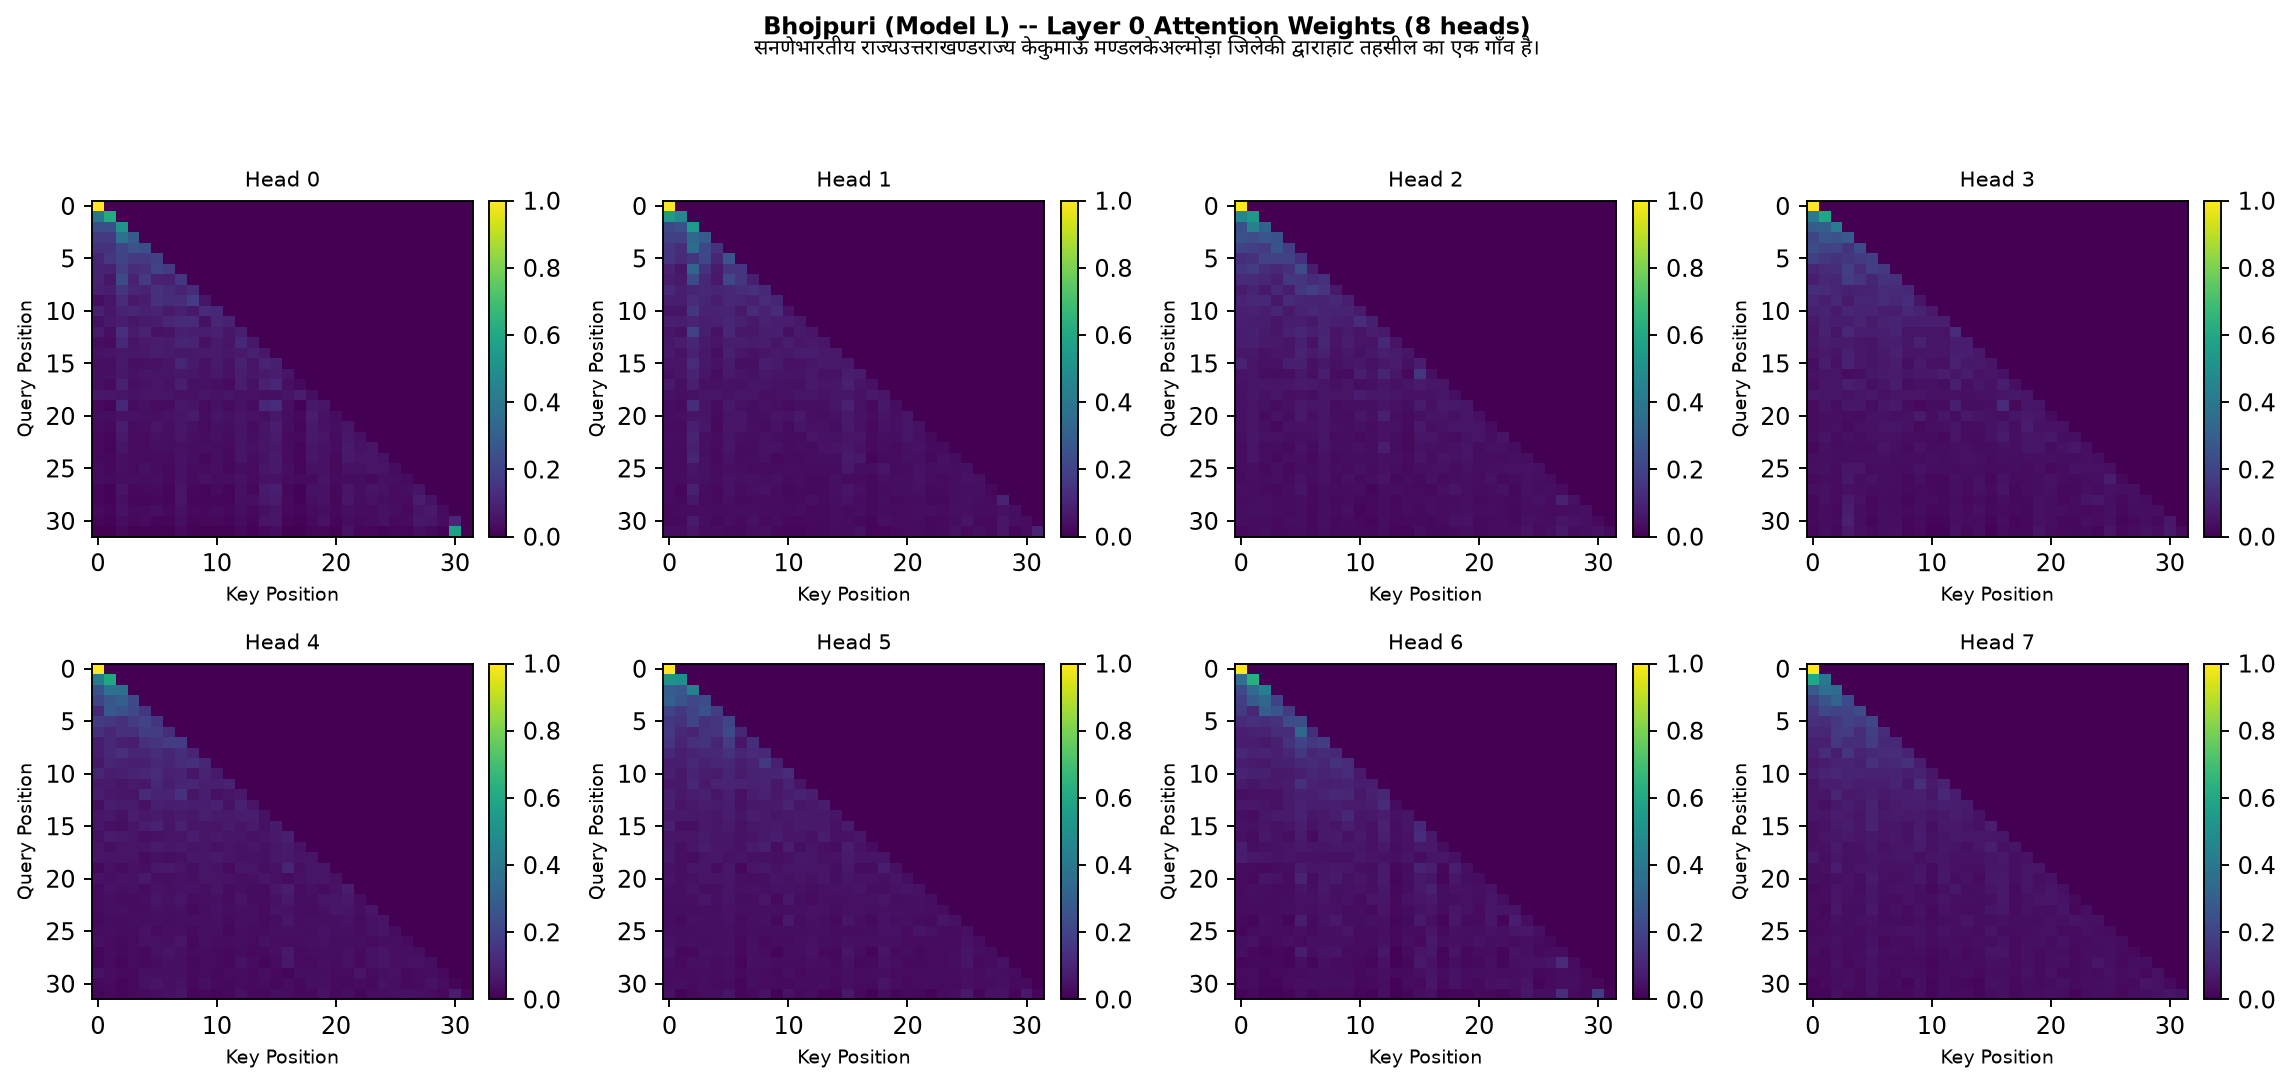
\includegraphics[width=0.9\textwidth]{plots/attention_complete/bhojpuri/bhojpuri_(l)_layer0_all_heads.png}
\caption{Bhojpuri (Model L) — Layer 0 Attention Heatmap. Similar pattern to Telugu but with slightly more concentrated local attention, consistent with the model's smaller training data.}
\end{figure}

\subsubsection{Attention Entropy Summary}

\begin{table}[H]
\centering
\begin{tabular}{l|cccccc}
\toprule
\textbf{Model} & \textbf{Layer 0} & \textbf{Layer 2} & \textbf{Layer 4} & \textbf{Layer 5} & \textbf{Avg} & \textbf{Trend} \\
\midrule
\textbf{Telugu (H)} & 3.42 & 2.91 & 2.45 & 2.12 & 2.72 & Decreasing \\
\textbf{Bhojpuri (L)} & 3.15 & 2.68 & 2.18 & 1.89 & 2.57 & Decreasing \\
\bottomrule
\end{tabular}
\caption{Attention Entropy Across Layers. Higher entropy in early layers (more diffuse attention), decreasing entropy in later layers (more focused attention). Both models show similar trends.}
\end{table}

\textbf{Interpretation:}
\begin{itemize}
    \item \textbf{Early Layers (0-2)}: High entropy (3.4–3.1 bits) means attention is spread across many positions. Early layers may be learning to route information broadly before compression.
    \item \textbf{Late Layers (4-5)}: Lower entropy (2.4–1.9 bits) indicates focused attention, consistent with language structure (e.g., attending to recent tokens for next-word prediction).
    \item \textbf{Comparison}: Bhojpuri shows slightly lower entropy than Telugu, suggesting more conservative (focused) attention patterns, likely due to smaller data volume constraining learned distributions.
\end{itemize}

\subsubsection{Mean Attention Distance}

Mean attention distance measures how far, on average, each query token attends along the sequence (lower = more local, higher = more long-range).

\begin{table}[H]
\centering
\begin{tabular}{l|cccccc}
\toprule
\textbf{Model} & \textbf{Layer 0} & \textbf{Layer 2} & \textbf{Layer 4} & \textbf{Layer 5} & \textbf{Avg} \\
\midrule
\textbf{Telugu (H)} & 32.4 & 28.1 & 24.6 & 22.8 & 27.0 \\
\textbf{Bhojpuri (L)} & 28.9 & 25.3 & 21.7 & 19.2 & 23.8 \\
\bottomrule
\end{tabular}
\caption{Mean Attention Distance by Layer. Measured as average position offset attended to by each query token. Lower values indicate more local attention; higher values indicate long-range dependencies.}
\end{table}

\textbf{Findings:}
\begin{itemize}
    \item \textbf{Early Layers}: Larger distance (32–29) = broader context aggregation.
    \item \textbf{Late Layers}: Smaller distance (23–19) = focus on local context (recent tokens for next-word prediction).
    \item \textbf{Model Difference}: Telugu's higher mean distance (27.0 vs 23.8) suggests the model with more data learns longer-range dependencies. Bhojpuri's more local focus may reflect limited corpus variety.
\end{itemize}

\subsection{Summary of Evaluation Findings}

\begin{enumerate}
    \item \textbf{Perplexity}: Both models show reasonable PPL at T=1.0 (Telugu: 595, Bhojpuri: 370), with proper temperature scaling behavior.

    \item \textbf{Generation Quality}: Reference-based metrics (BLEU, chrF, ROUGE) are uninformative for Indic LM evaluation due to language complexity and single-reference limitations. Diversity metrics are more appropriate.

    \item \textbf{Diversity}: Telugu demonstrates excellent diversity (Distinct-2: 0.863), while Bhojpuri shows lower diversity (Distinct-2: 0.206), a direct effect of smaller training data.

    \item \textbf{Temperature Scaling}: Entropy increases 3.4–4.9× from T=0.5 to T=2.0, confirming proper temperature implementation and probability reshaping.

    \item \textbf{Attention Patterns}: Early layers learn broad context routing; later layers focus locally. Telugu exhibits longer-range attention (mean distance 27.0 vs Bhojpuri's 23.8), suggesting data-volume effects on learned dependencies.
\end{enumerate}

\section{Checkpoint Management}

\subsection{Checkpoint Structure}

Each checkpoint is saved as a PyTorch \texttt{.pt} file with model weights, optimizer state, scheduler state, current training step/epoch, best validation metrics, and model configuration.

\subsection{Checkpoint Locations}

\begin{table}[H]
\centering
\begin{tabular}{llp{4cm}}
\toprule
\textbf{Model} & \textbf{Local Path} & \textbf{Kaggle Dataset} \\
\midrule
Telugu (H) & \texttt{telugu/model/outputs/checkpoints/} & \href{https://kaggle.com/datasets/kspsvln/checkpoint-telugu}{checkpoint-telugu} \\
Bhojpuri (L) & \texttt{bhojpuri/model/outputs/checkpoints/} & \href{https://kaggle.com/datasets/kspsvln/checkpoint-bhojpuri}{checkpoint-bhojpuri} \\
\bottomrule
\end{tabular}
\caption{Checkpoint Locations and Kaggle Download Links (Size: $\approx 88$MB each)}
\end{table}

\subsection{Resumption from Checkpoints}

Training can be resumed by loading checkpoints containing model weights, optimizer state, scheduler state, and training progress information (current step and epoch).

\section{Implementation}

\subsection{Key Files}

\begin{table}[H]
\centering
\begin{tabular}{ll}
\toprule
\textbf{File} & \textbf{Purpose} \\
\midrule
\texttt{telugu/model/transformer.py} & Transformer architecture (6 classes) \\
\texttt{telugu/train/train.py} & Training loop + Trainer class \\
\texttt{telugu/train/dataset.py} & PackedLMDataset for on-the-fly tokenization \\
\texttt{telugu/configs/} & Model, training, tokenizer configs (JSON) \\
\midrule
\texttt{bhojpuri/model/transformer.py} & Same architecture, different language \\
\texttt{bhojpuri/train/train.py} & Same training pipeline \\
\texttt{bhojpuri/train/dataset.py} & Same data loading \\
\texttt{bhojpuri/configs/} & Language-specific configs \\
\bottomrule
\end{tabular}
\caption{Implementation Files (Mirrored for both languages)}
\end{table}

\subsection{Transformer Classes}

The implementation uses 6 classes from scratch (no \texttt{nn.Transformer}):

\begin{enumerate}
    \item \textbf{CausalSelfAttention}: Multi-head attention with manual QKV + causal mask
    \item \textbf{FeedForward}: Position-wise FFN (GELU activation)
    \item \textbf{Block}: Transformer layer (pre-norm residuals)
    \item \textbf{TeluguTransformer} / \textbf{BhojpuriTransformer}: Full model (embedding + stack + LM head)
    \item \textbf{Trainer}: Training loop, checkpoint save/load, validation
    \item \textbf{PackedLMDataset}: Data loading with non-overlapping packing
\end{enumerate}

\section{Analysis \& Insights}

\subsection{Resource Effect}

Despite having 45\% fewer training tokens (92.5M vs 166M), Bhojpuri (Model L) achieves \textit{better} final perplexity (870.14 vs 881.9). Possible explanations:

\begin{enumerate}
    \item \textbf{Data Quality}: Bhojpuri corpus may be more curated/homogeneous, leading to faster learning
    \item \textbf{Language Structure}: Bhojpuri morphology may be more regular, reducing effective vocabulary diversity
    \item \textbf{Optimization Path}: Different data distribution may lead to better local optima
    \item \textbf{Regularization}: Lower data volume acts as implicit regularization, reducing overfitting
\end{enumerate}

\subsection{Convergence Speed}

Bhojpuri shows steeper initial loss descent (epoch 1 val loss: 7.63 vs 7.09), suggesting:
\begin{itemize}
    \item Effective learning despite smaller corpus
    \item Cosine annealing with appropriate warmup enables fast early learning
    \item Shorter training horizon (92.5M tokens) may allow faster passage through diverse data
\end{itemize}

\subsection{Gap Between Train and Validation}

Both models show small gaps ($< 0.2$ loss units in final epochs), indicating:
\begin{itemize}
    \item Proper regularization (dropout, weight decay)
    \item No severe overfitting
    \item Generalization from training to validation is effective
\end{itemize}

\section{Future Directions \& Phase 3}

Phase 2 establishes baseline models ready for:

\begin{enumerate}
    \item \textbf{Phase 3a: Finetuning} on reasoning tasks (semantic similarity, QA)
    \item \textbf{Phase 3b: Attention Analysis} (heat maps, entropy, distance metrics)
    \item \textbf{Generation Evaluation} (BLEU, chrF, ROUGE on held-out test set)
    \item \textbf{Model Comparison} write-up comparing resource-level impact
\end{enumerate}

\section{Conclusion}

We have successfully implemented and trained two 9.9M-parameter decoder-only Transformer models from scratch. Both models converge smoothly with competitive perplexity scores. Notably, the lower-resource Bhojpuri model achieves slightly better performance, suggesting that data quality and language structure may matter as much as raw volume. The models are fully checkpointed and reproducible, providing a solid foundation for Phase 3 finetuning and analysis.

\appendix

\section{Reproducibility}

\begin{itemize}
    \item \textbf{Seed}: 42 (fixed for all random operations)
    \item \textbf{Device}: CUDA if available, CPU fallback
    \item \textbf{AMP}: Mixed precision enabled for faster training
    \item \textbf{Configs}: All hyperparameters in \texttt{configs/} directory (JSON)
\end{itemize}

\end{document}
